\section{Dynamic Documents For Computational
Reproducibility}\label{dynamic-documents-for-computational-reproducibility}

\begin{frame}[fragile]{Dynamic Documents For Computational
Reproducibility}

\begin{itemize}
\tightlist
\item
  Based on principles of \emph{literate programming} aims at combining
  code and paper in one single document
\item
  Best framework to achieve the holy grail of \textbf{one-click
  reproducible workflow}
\item
  Best two current implementations: \texttt{RMarkdown\ (R)} \&
  \texttt{Jupyter\ (Python)}. \texttt{Stata} is catching up (more at the
  end)
\end{itemize}

\end{frame}

\begin{frame}{Currently code and narrative components live in separate
universes}

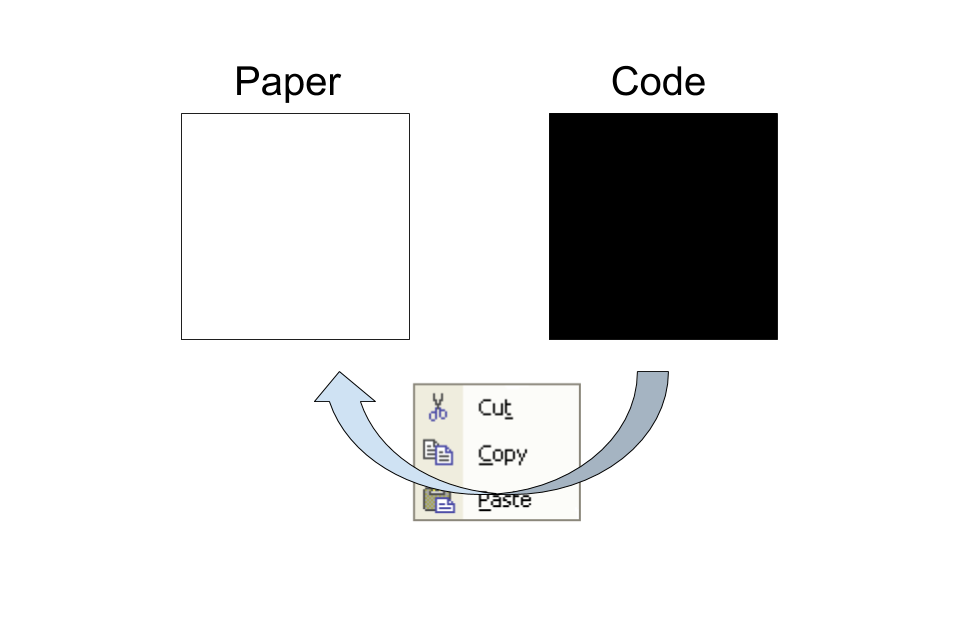
\includegraphics{./Two universes.png}

\end{frame}

\begin{frame}{Dynamic Documents: integrate the two universes!}


\includegraphics{./One universe.png}

\end{frame}

\begin{frame}[fragile]{Dynamic Documents: A Recipe}

\begin{itemize}
\tightlist
\item
  1 simple language that can combine text and code: \texttt{Markdown}
\item
  1 statistical package to do the analysis (\texttt{R}, \texttt{Python},
  \texttt{3S\textquotesingle{}s?})
\item
  1 machinery to combine analysis and text to create a single output:
  \texttt{Pandoc}
\item
  {[}Optional-but-not-really{]} 1 program to bring all the elements
  together: RStudio/RMarkdown, Jupyter
\end{itemize}

\end{frame}

\begin{frame}{Markdown laguange/syntax in 60 seconds}

\includegraphics{./RStudioCS.png}

\end{frame}

\section{One Type of Dynamic Document: R
Markdown}\label{one-type-of-dynamic-document-r-markdown}

\begin{frame}[fragile]{For our excercise: R Markdown}

\begin{itemize}
\tightlist
\item
  \texttt{R}: \textbf{open source} programming language design for
  statistical analysis.\\
\item
  RStudio: free software that provides and Integrated Development
  Environment (IDE)\\
\item
  RStudio combines all together: R + Markdown + Pandoc to produce
  multiple outputs
  \includegraphics{http://rmarkdown.rstudio.com/images/RMarkdownFlow.png}
\end{itemize}

\end{frame}

\begin{frame}{R Markdown}

\includegraphics{http://rmarkdown.rstudio.com/images/RMarkdownOutputFormats.png}

\end{frame}

\begin{frame}{Basic Structure}

\begin{itemize}
\tightlist
\item
  A header
\item
  Text
\item
  Code: inline and chunks
\end{itemize}

\end{frame}

\begin{frame}[fragile]{Basic Structure: Header}

\begin{Shaded}
\begin{Highlighting}[]
\OperatorTok{---}
\NormalTok{title}\OperatorTok{:}\StringTok{ "Sample Paper"}
\NormalTok{author}\OperatorTok{:}\StringTok{ "Fernando Hoces de la Guardia"}
\NormalTok{output}\OperatorTok{:}\StringTok{ }\NormalTok{html_document}
\OperatorTok{---}
\end{Highlighting}
\end{Shaded}

\end{frame}

\begin{frame}[fragile]{Basic Structure: Body of Text}

\begin{Shaded}
\begin{Highlighting}[]
\OperatorTok{---}
\NormalTok{header}
\OperatorTok{---}
\end{Highlighting}
\end{Shaded}

This is where you write your paper. Nothing much to add. You can check
Markdown
\href{https://www.rstudio.com/wp-content/uploads/2015/02/rmarkdown-cheatsheet.pdf}{syntax
here}. And it can use can type equations using LaTex syntax!

\end{frame}

\begin{frame}[fragile]{Basic Structure: Code Chunks and Inline}

\begin{Shaded}
\begin{Highlighting}[]
\OperatorTok{---}
\NormalTok{header}
\OperatorTok{---}
\end{Highlighting}
\end{Shaded}

Body of text.

To begin a piece of code (``code chunk''). Enclose them in the following
expression (Ctrl/Cmd + shift/optn + i)

\begin{verbatim}
```{r, eval=TRUE}
here goes the code
```
\end{verbatim}

To write inline use only one Backtick to open followed by an ``r''" and
one to close \texttt{\textasciigrave{}r\ 1+1\textasciigrave{}} in the
output.

\end{frame}

\section{Practical Excercise \#1}\label{practical-excercise-1}

\begin{frame}{Hands-on excercise: the birthday problem!}

As an illustration lets write a report using the participants in this
workshop to illustrate the famous
\href{https://en.wikipedia.org/wiki/Birthday_problem}{birthday problem}.

\begin{quote}
What is the probability that at least two people this room share the
same birthday?
\end{quote}

\begin{quote}
Is it something like \(\frac{1}{365} \times N =\) 0.11?
\end{quote}

\end{frame}

\begin{frame}[fragile]{Create a new RMarkdown File}

1 - In RStudio:
\texttt{File-\textgreater{}\ New\ File\ -\textgreater{}\ RMarkdown...}\\
2 - Name it, and save it.\\
3 - Review/edit the header, and delete all the default body of text
except for one code chunk.\\
4 - Define a seed (\texttt{set.seed\ =\ 1234} and number of people in
the room (\texttt{n.pers\ =\ ?})

\end{frame}

\begin{frame}{The birthday problem: the math}

Actually the math says otherwise:

\begin{align} 
 1 - \bar p(n) &= 1 \times \left(1-\frac{1}{365}\right) \times \left(1-\frac{2}{365}\right) \times \cdots \times \left(1-\frac{n-1}{365}\right) \nonumber  \\  &= \frac{ 365 \times 364 \times \cdots \times (365-n+1) }{ 365^n } \nonumber \\ &= \frac{ 365! }{ 365^n (365-n)!} = \frac{n!\cdot\binom{365}{n}}{365^n}\\
p(n= 40) &= 0.891  \nonumber
\end{align}

\end{frame}

\begin{frame}[fragile]{Code for the math (\url{https://goo.gl/cf3w1Y})}

Don't look at this: just copy and paste into your report

\begin{Shaded}
\begin{Highlighting}[]
\NormalTok{\textbackslash{}begin\{align\} }
 \DecValTok{1} \OperatorTok{-}\StringTok{ }\NormalTok{\textbackslash{}bar }\KeywordTok{p}\NormalTok{(n) }\OperatorTok{&}\ErrorTok{=}\StringTok{ }\DecValTok{1}\NormalTok{ \textbackslash{}times \textbackslash{}}\KeywordTok{left}\NormalTok{(}\DecValTok{1}\OperatorTok{-}\NormalTok{\textbackslash{}frac\{}\DecValTok{1}\NormalTok{\}\{}\DecValTok{365}\NormalTok{\}}
\NormalTok{                                 \textbackslash{}right) }
\NormalTok{ \textbackslash{}times \textbackslash{}}\KeywordTok{left}\NormalTok{(}\DecValTok{1}\OperatorTok{-}\NormalTok{\textbackslash{}frac\{}\DecValTok{2}\NormalTok{\}\{}\DecValTok{365}\NormalTok{\}\textbackslash{}right) \textbackslash{}times \textbackslash{}cdots }
\NormalTok{ \textbackslash{}times }
\NormalTok{ \textbackslash{}}\KeywordTok{left}\NormalTok{(}\DecValTok{1}\OperatorTok{-}\NormalTok{\textbackslash{}frac\{n}\OperatorTok{-}\DecValTok{1}\NormalTok{\}\{}\DecValTok{365}\NormalTok{\}\textbackslash{}right) \textbackslash{}nonumber  \textbackslash{}\textbackslash{}  }
 \OperatorTok{&}\ErrorTok{=}\StringTok{ }\NormalTok{\textbackslash{}frac\{ }\DecValTok{365}\NormalTok{ \textbackslash{}times }\DecValTok{364}\NormalTok{ \textbackslash{}times \textbackslash{}cdots \textbackslash{}times }
\NormalTok{   (}\DecValTok{365}\OperatorTok{-}\NormalTok{n}\OperatorTok{+}\DecValTok{1}\NormalTok{) \}\{ }\DecValTok{365}\OperatorTok{^}\NormalTok{n \} \textbackslash{}nonumber \textbackslash{}\textbackslash{} }
 \OperatorTok{&}\ErrorTok{=}\StringTok{ }\NormalTok{\textbackslash{}frac\{ }\DecValTok{365}\OperatorTok{!}\StringTok{ }\NormalTok{\}\{ }\DecValTok{365}\OperatorTok{^}\KeywordTok{n}\NormalTok{ (}\DecValTok{365}\OperatorTok{-}\NormalTok{n)}\OperatorTok{!}\NormalTok{\} =}\StringTok{ }
\StringTok{   }\NormalTok{\textbackslash{}frac\{n}\OperatorTok{!}\NormalTok{\textbackslash{}cdot\textbackslash{}binom\{}\DecValTok{365}\NormalTok{\}\{n\}\}\{}\DecValTok{365}\OperatorTok{^}\NormalTok{n\}\textbackslash{}\textbackslash{}}
\KeywordTok{p}\NormalTok{(}\DataTypeTok{n=} \StringTok{`}\DataTypeTok{r n.pers}\StringTok{`}\NormalTok{) }\OperatorTok{&}\ErrorTok{=}\StringTok{ `}\DataTypeTok{r  }
\DataTypeTok{ round(1 - factorial(n.pers) * }
\DataTypeTok{         choose(365,n.pers)/ 365^n.pers, 3)}\StringTok{`}
\NormalTok{ \textbackslash{}nonumber}
\NormalTok{\textbackslash{}end\{align\}}
\end{Highlighting}
\end{Shaded}

\end{frame}

\begin{frame}{Don't like math? Let's run a simple simulation!}

1 - Simulate 10,000 rooms with \(n = 40\) random birthdays, and store
the results in matrix where each row represents a room.\\
2 - For each room (row) compute the number of unique birthdays.\\
3 - Compute the average number of times a room has 40 unique birthdays,
across 10,000 simulations, and report the complement.

\end{frame}

\begin{frame}[fragile]{Code for the simulation
(\url{https://goo.gl/cf3w1Y})}

\begin{Shaded}
\begin{Highlighting}[]
\NormalTok{birthday.prob =}\StringTok{ }\ControlFlowTok{function}\NormalTok{(n.pers, n.sims) \{}
  \CommentTok{# simulate birthdays}
\NormalTok{  birthdays =}\StringTok{ }\KeywordTok{matrix}\NormalTok{(}\KeywordTok{round}\NormalTok{(}\KeywordTok{runif}\NormalTok{(n.pers }\OperatorTok{*}\StringTok{ }\NormalTok{n.sims, }
                                 \DecValTok{1}\NormalTok{, }\DecValTok{365}\NormalTok{)), }
                      \DataTypeTok{nrow =}\NormalTok{ n.sims, }\DataTypeTok{ncol =}\NormalTok{ n.pers)}
  \CommentTok{# for each room (row) get unique birthdays}
\NormalTok{  unique.birthdays =}\StringTok{ }\KeywordTok{apply}\NormalTok{(birthdays, }\DecValTok{1}\NormalTok{, unique)}
  \CommentTok{# Indicator with 1 if all are unique birthdays}
\NormalTok{  all.different =}\StringTok{ }\NormalTok{(}\KeywordTok{lapply}\NormalTok{(unique.birthdays, }
\NormalTok{                          length) }\OperatorTok{==}\StringTok{ }\NormalTok{n.pers)}
  \CommentTok{# Compute average time all have different birthdays }
\NormalTok{  result =}\StringTok{ }\DecValTok{1} \OperatorTok{-}\StringTok{ }\KeywordTok{mean}\NormalTok{(all.different)}
\KeywordTok{return}\NormalTok{(result)}
\NormalTok{\}}
\NormalTok{n.pers.param =}\StringTok{ }\DecValTok{40}
\NormalTok{n.sims.param =}\StringTok{ }\FloatTok{1e4}
\KeywordTok{birthday.prob}\NormalTok{(n.pers.param,n.sims.param)}
\end{Highlighting}
\end{Shaded}

\begin{verbatim}
## [1] 0.8928
\end{verbatim}

\end{frame}

\begin{frame}{Results}

\begin{itemize}
\tightlist
\item
  Many people originally think of a prob \textasciitilde{}
  \(\frac{1}{365} \times N =\) 0.11
\item
  However the true probability is of \(p(n= 40) = 0.891\)
\item
  And the simulated probability is of 0.8928
\end{itemize}

\end{frame}

\section{Practical Excercise \#2}\label{practical-excercise-2}

\begin{frame}{Hands-on excercise \#2: Mostly Harmless Econometrics!
(@WB?)}

There is a
\href{https://github.com/vikjam/mostly-harmless-replication}{fantastic
Github} repo that is reproducing results from MHE (Originated here?)

Lets use the of examples Figure
\href{https://github.com/vikjam/mostly-harmless-replication/blob/master/05\%20Fixed\%20Effects\%2C\%20DD\%20and\%20Panel\%20Data/Figure\%205-2-4.r}{5.2.4}
to show how dynamic docs can be used in data analysis.

\end{frame}

\section{Final Remarks \& More
Resources}\label{final-remarks-more-resources}

\begin{frame}{Final Remarks \& More Resources}

\begin{itemize}
\tightlist
\item
  With DD we can achieve a one-click reproducible workflow.
\item
  This is particularly helpful to understand/present results that are
  hard to digest.
\item
  Stata just develop an internal version of DD for v15.
  \href{https://www.bitss.org/2017/09/05/review-of-statas-dyndoc/}{Review
  Here}
\item
  More great examples
  \href{https://github.com/BITSS/Annual2017/tree/master/3-Rmarkdown}{here}
\item
  Want to learn more: \href{https://bookdown.org/}{great free books}
  (can you guess how they were written?)
\end{itemize}

\end{frame}
